\section{Redundant Array of Independent Disks}

Redundant Arrays of Independent Disks (RAID) is a storage technology introduced in the 1980s by Patterson. 
Its purpose is to enhance the performance, capacity, and reliability of storage systems. 
RAID achieves this by combining multiple independent disks into a single logical unit with improved performance.

This approach stands in contrast to Just a Bunch of Disks (JBOD), where each disk functions as a separate entity with its own mount point.
Instead, RAID stripes data across several disks, allowing for parallel access. 

RAID employs two primary techniques: data striping to boost performance and redundancy to enhance reliability. 
These orthogonal methods work together to provide improved storage capabilities for various computing needs.

The distribution of data in RAID systems is facilitated through I/O virtualization.
This means that data is distributed transparently across the disks, requiring no action from the users. 

\paragraph*{Data striping}
Data striping in RAID involves writing data sequentially, such as vectors, files, or tables, onto multiple disks in units called stripes. 
These stripes can be defined by various units, such as bits, bytes, or blocks, and are written according to a cyclic algorithm, typically a round-robin approach.

The stripe unit refers to the size of the data unit that is written on a single disk, while the stripe width indicates the number of disks considered by the striping algorithm.

There are several benefits to data striping:
\begin{itemize}
    \item Multiple independent I/O requests can be executed in parallel by several disks.
    \item Single multiple-block I/O requests can be executed by multiple disks in parallel.
\end{itemize}

\paragraph*{Redundancy}
Redundancy in RAID serves as a safeguard against data loss in the event of disk failure. 
By duplicating or distributing data across multiple disks in a redundant manner, the system can withstand the failure of one or more disks without losing critical data. 
Redundancy mechanisms such as mirroring (RAID 1), parity (RAID 5), or both (RAID 6) provide fault tolerance and ensure data integrity even in the face of hardware failures.

\paragraph*{Performance}
In redundancy-based RAID configurations, error correcting codes are computed and stored on disks separate from those holding the primary data. 
These error correcting codes provide the ability to tolerate data loss resulting from disk failures. 
However, the implementation of redundancy introduces overhead in terms of performance, particularly during write operations.

During write operations, updates must also be made to the redundant information, which results in a performance penalty compared to traditional writes. 
This is because the additional computation and storage required for redundancy checking and updating the error correcting codes increase the time required to complete write operations.

\paragraph*{Update consistency}
Mirrored writes should be atomic, meaning that all copies are written, or none are written.
However, this is difficult to guarantee.
Many RAID controllers include a write-ahead log, which is a battery-backed, non-volatile storage of pending writes. 
A recovery procedure ensures that the out-of-sync mirrored copies are recovered.













\subsection{RAID 0}

Data is inscribed onto a solitary logical disk and partitioned into multiple blocks dispersed across disks based on a striping algorithm. 
This method is preferred when prioritizing performance and capacity over reliability, necessitating a minimum of two drives. 
It offers cost-effectiveness since redundancy isn't utilized, meaning error-correcting codes aren't calculated or stored. 
It excels in write performance due to the absence of redundant data updates and parallelization.
However, a single disk failure can lead to irreversible data loss.

\subsection{Striping}
The core concept behind striping is to depict an array of disks as a unified large disk, thus maximizing parallelism by distributing data across all $N$ disks.
\begin{figure}[H]
    \centering
    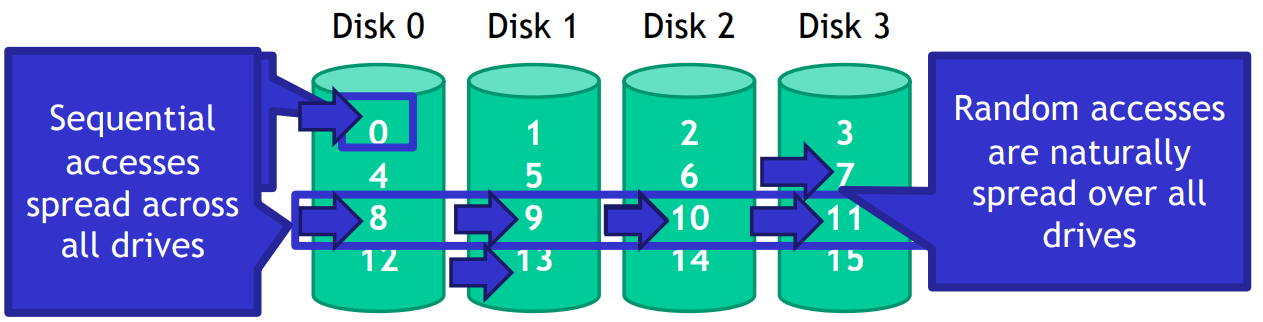
\includegraphics[width=0.4\linewidth]{images/strip.png}
    \caption{Data striping}
\end{figure}
Sequential accesses are evenly distributed across all drives, while random accesses occur naturally across all drives as well.
The access to a specific data blocks can be done by computing the number of disk, and the offset: 
\[\text{Disk}=\text{logical block number} \% \text{number of disks}\]
\[\text{Disk}=\dfrac{\text{logical block number}}{\text{number of disks}}\]

\paragraph*{Chunk sizing}
Chunk size influences array performance:
\begin{itemize}
    \item Smaller chunks lead to increased parallelism.
    \item Larger chunks result in reduced seek times.
\end{itemize}
Typical arrays utilize 64 kilobytes chunks.

\subsection{Summary}
The following is a summary of the features of RAID 0:
\begin{itemize}
\item The system has a capacity of $N$, meaning that it can hold all of the data on all drives.
\item The system has a reliability of $0$, meaning that if any drive fails, data will be permanently lost. 
    The Mean Time to Data Loss is equal to the Mean Time to Failure.
\item The system supports sequential read and write operations of $N\times S$, which means that data can be read and written in parallel across all drives.
\item The system also supports random read and write operations of $N\times R$, which means that data can be read and written in a random pattern across all drives.
\end{itemize}




\subsection{RAID 1}
RAID one is a type of data storage configuration where data is duplicated (mirrored) to a second disk. 
This provides high reliability, as when a disk fails, the second copy can be used. 
Reads of data can be retrieved from the disk with shorter queueing, seek, and latency delays.
However, writes are slower than standard disks due to the duplication, and the cost of using 50\% of the capacity is higher.

In principle, a RAID 1 can mirror the content over more than one disk. 
This provides resiliency to errors even if more than one disk breaks.
Additionally, with a voting mechanism, it allows for the identification of errors not reported by the disk controller. 
However, in practice, this is never used because the overhead and costs are too high.

\subsection{Mirroring}
The key idea for mirroring is to make two copies of all data. 
This provides data redundancy, which means that if one copy of the data is lost or corrupted, the other copy can be used to recover the data. 
This provides a level of fault tolerance and data protection that is not present in RAID 0, which offers high performance but no error recovery.
By making two copies of all data, mirroring provides both high performance and data protection.

If multiple disks are available, they can be coupled in an even number to achieve a total capacity that is halved. 
Each disk can have a mirror, and RAID levels can be combined to achieve the desired performance and redundancy. 
The two possible combinations are RAID $01$ and RAID $10$.

\subsection{Multiple levels RAID}
RAID levels can be combined by considering the number of groups of disks and applying RAID $x$ to each group of $n$ disks. 
Then, RAID $y$ can be applied to the $m$ groups of $n$ disks, resulting in a total of $n \times m$ disks.
\begin{figure}[H]
    \centering
    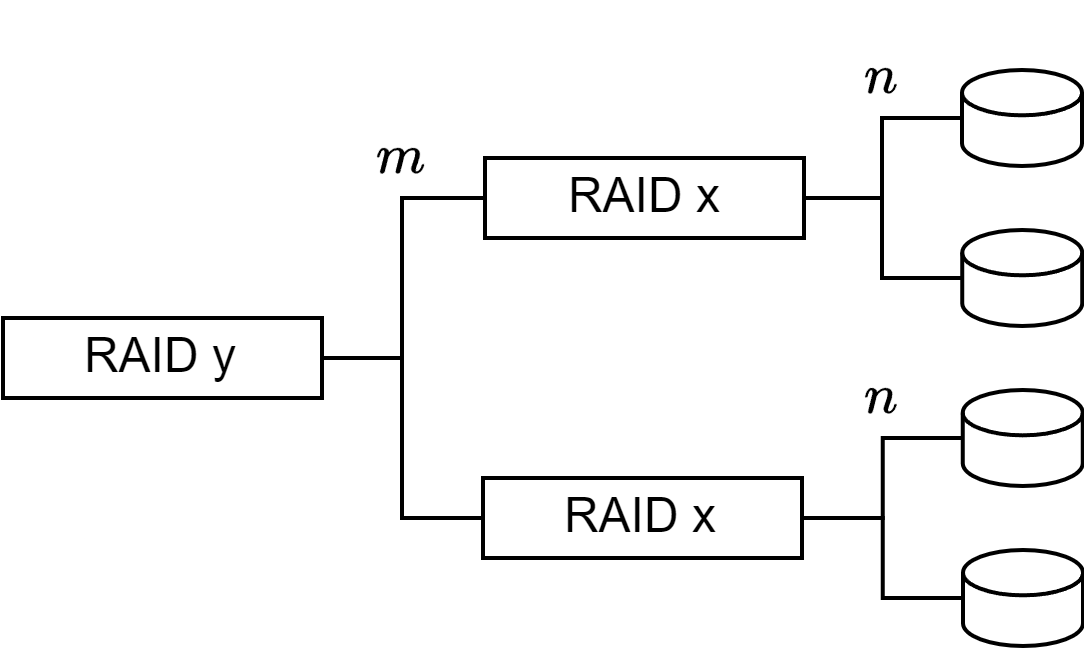
\includegraphics[width=0.5\linewidth]{images/level.png}
    \caption{RAID levels}
\end{figure}

\paragraph*{RAID 01}
RAID level 0 + 1 is a type of RAID (Redundant Array of Independent Disks) configuration where data is first striped across multiple drives using RAID 0, and then mirrored using RAID 1. 
This provides both high performance and data redundancy. 
In the event of a failure of one of the drives in the RAID 0 stripe, the data is still available on the other drives, and the RAID 1 mirror provides an additional copy of the data for protection. 
The minimum number of drives required for this configuration is four.

\paragraph*{RAID 10}
RAID 10 is a type of RAID (Redundant Array of Independent Disks) level that combines the mirroring of RAID 1 with the striping of RAID 0. 
In RAID 10, data is first mirrored across two or more drives (RAID 1), and then the mirrored data is striped across the remaining drives (RAID 0). 
This provides both data redundancy and improved performance for read and write operations.
RAID 10 is commonly used in databases with very high workloads, particularly those that require fast writes.
A minimum of four drives are required to implement RAID 10.

\subsection{Comparison}
RAID 0, 1, 0+1, and 1+0 organizations differ in the order of block allocation.
Both RAID 10 and RAID 01 have the same performance. 
The storage capacity of RAID 10 and RAID 01 is the same.
The main difference between these RAID organizations is their fault tolerance levels:
\begin{itemize}
    \item RAID 0+1 has less fault tolerance on most RAID controller implementations.
    \item RAID 1+0 has a larger fault tolerance level.
\end{itemize}

\subsection{Summary}
The following is a summary of the features of RAID 1:
\begin{itemize}
    \item The system has a capacity of $\frac{N}{2}$, meaning it can store half of the total data.
    \item The system has a reliability of $1$, meaning that if one drive fails, the system can still function without data loss.
        However, if multiple drives fail, the system may not be able to recover all of the data. 
        In the best-case scenario, $\frac{N}{2}$ drives can fail without data loss.
    \item The system supports sequential read and write operations of $\frac{N}{2}\times S$, which means that it can read and write half of the data in the system at a time.
        This results in a throughput of $\frac{N}{2}\times S$.
    \item The system also supports random read and write operations of $\frac{N}{2}\times R$, which means that it can read and write half of the read blocks in the system at a time. 
        However, since only half of the read blocks are actually being read, this results in half of the read throughput.
\end{itemize}
In the best scenario, it is possible to have $\frac{N}{2} \times R$ random writes, where $N$ is the number of disks and $R$ is the number of random writes per disk. 
This is because we have two copies of all data, so the throughput is halved. 
On the other hand, reads can parallelize across all disks, so it is possible to have $N \times R$ random reads in the best scenario.

\subsection{RAID 4}

In RAID four, the $N$-th disk only stores parity information for the other $N-1$ disks. 
The parity bit is computed using the XOR operation.

\paragraph*{Writes}
There are two methods for updating parity when blocks are written:
\begin{itemize}
    \item Additive parity involves reading other blocks and then updating the parity block. 
        This method calculates the new parity value by XORing the old parity value with the new parity value.
    \item Subtractive parity involves updating the disk and then computing the new parity value. 
        This method calculates the new parity value by XORing the old parity value with the new parity value.
\end{itemize}

\paragraph*{Reads}
In RAID 4, reads are not a problem because the data is distributed evenly across all non-parity blocks in the stripe. 
This ensures that read operations can be performed efficiently without any significant performance reduction due to the parity disk.

RAID 4 has the same read and write performance, with parallelization across all non-parity blocks in the stripe. 
This means that all writes on the same stripe update the parity drive once.

\paragraph*{Random writes}
In RAID 4, random writes can cause a bottleneck due to the need to update the parity drive, which can cause serialization. 
The process of writing to a RAID 4 array involves reading the target block and the parity block, calculating the new parity block using subtraction, and then writing the target block and the new parity block. 
This process can cause performance issues, especially if the parity drive is slow or has limited bandwidth.

\subsection{Summary}
The following is a summary of the features of RAID 1:
\begin{itemize}
    \item The system has a capacity of $N-1$, meaning that the space on the parity drive is lost. 
    \item The system has a reliability of $1$, meaning that one drive can fail. 
        This can result in massive performance degradation during a partial outage.
    \item The system supports sequential read and write operations of $(N-1)\times S$, which means that it can perform parallelization across all non-parity blocks in the stripe.
    \item The system supports parallelization of read operations over all drives except the parity drive, with a maximum of $(N-1)\times R$ simultaneous reads.
    \item The system supports random write operations of $\frac{R}{2}$, which means that writes serialize due to the parity drive. 
        Each write requires one read and one write of the parity drive.
\end{itemize}


\subsection{RAID 5}

In RAID 5, the parity blocks are distributed evenly across all N disks. 
Unlike RAID 4, writes are spread evenly across all drives.
Random writes in RAID 5 involve the following steps:
\begin{enumerate}
    \item Read the target block and the parity block.
    \item Calculate the new parity block by subtracting the old parity block from the target block.
    \item Write the target block and the new parity block.
\end{enumerate}
This results in a total of 4 operations (2 reads and 2 writes) being distributed evenly across all drives.

\subsection{Summary}
The following is a summary of the features of RAID 1:
\begin{itemize}
    \item The system has a capacity of $N-1$, meaning that the space on the parity drive is lost. 
    \item The system has a reliability of $1$, meaning that one drive can fail. 
        This can result in massive performance degradation during a partial outage.
    \item The system supports sequential read and write operations of $(N-1)\times S$, which means that it can perform parallelization across all non-parity blocks in the stripe.
    \item The system supports parallelization of read operations over all drives, with a maximum of $N\times R$ simultaneous reads.
    \item The system supports random write operations of $\frac{N}{4}R$, which means that writes parallelize over all drives. 
        Each write requires two reads and two writes. 
\end{itemize}

\subsection{RAID 6}

RAID 6 is a type of RAID level that provides more fault tolerance than RAID 5. 
It allows for two concurrent failures to be tolerated, which means that if two of the disks in the array fail, the data can still be recovered from the remaining disks. 
RAID 6 uses Solomon-Reeds codes with two redundancy schemes, which means that there are two different ways to encode the data on the disks. 
The (P+Q) distribution is distributed and independent, which means that the parity blocks are spread across all the disks in the array. 
This provides a higher level of fault tolerance than RAID 5. To implement RAID 6, a minimum of four data disks and two parity disks are required. 
Each write operation requires six disk accesses, as the data must be written to both the P and Q parity blocks, which can result in slow writes.



\subsection{Comparison}
\begin{table}[H]
    \centering
    \begin{tabular}{|c|ccccc|}
    \hline
    \textbf{RAID} & \textbf{Capacity} & \textbf{Reliability} & \makecell{\textbf{Read write} \\\textbf{performance}} & \makecell{\textbf{Rebuild} \\\textbf{performance}} & \textbf{Applications}                 \\ \hline
    \textit{0}    & $100\%$           & N/A                  & Very good                       & Good                         & Non critical data                     \\
    \textit{1}    & $50\%$            & Excellent            & Very good, good                 & Good                         & Critical information                  \\
    \textit{5}    & $\dfrac{\left(N-1\right)}{N}$   & Good                 & Good, fair                      & Poor                         & Database                              \\
    \textit{6}    & $\dfrac{\left(N-2\right)}{N}$   & Excellent            & Very good, poor                 & Poor                         & Critical information                  \\
    \textit{01}   & $50\%$            & Excellent            & Very good, good                 & Good                         & \makecell{Critical information \\ with performance} \\ \hline
    \end{tabular}
\end{table}
Based on the context information provided, the best performance and most capacity can be achieved with RAID 0. 
This is because RAID 0 allows for the striping of data across multiple drives, which can significantly increase read and write speeds. 
However, it is important to note that RAID 0 does not provide any data redundancy or fault tolerance, so it is not recommended for use in critical data storage scenarios.

The greatest error recovery can be achieved with RAID 1 (1+0 or 0+1). This is because RAID 1 provides data redundancy by mirroring data across multiple drives. 
If one drive fails, the data can still be accessed from the other drives. 
However, it is important to note that RAID 1 can also result in a decrease in performance compared to RAID 0.

The balance between space, performance, and recoverability can be achieved with RAID 5. 
This is because RAID 5 provides a balance between the three by allowing for data striping across multiple drives while also providing some level of data redundancy. 
However, it is important to note that RAID 5 can also result in a decrease in performance compared to RAID 0.

\subsection{Hot spares}
Many RAID systems include a hot spare, which is an idle, unused disk installed in the system.
In the event of a drive failure, the array is immediately rebuilt using the hot spare, allowing for seamless data recovery and minimizing downtime.

\subsection{Implementation}
RAID is a data storage technology that allows multiple hard drives or solid-state drives to be combined into a single logical unit that can be accessed as if it were a single drive. 
RAID can be implemented in either hardware or software.

Hardware RAID is implemented using specialized hardware controllers that are built into the motherboard or a separate expansion card. 
Hardware RAID is generally faster and more reliable than software RAID, as it offloads the processing of managing the RAID array to dedicated hardware. 
However, migrating a hardware RAID array to a different hardware controller can be challenging and may not always work successfully.

On the other hand, software RAID is implemented using software drivers that run on the computer's central processing unit (CPU). 
Software RAID is simpler to migrate and cheaper than hardware RAID, but it has worse performance and weaker reliability due to the consistent update problem. 
This problem occurs because software RAID relies on the CPU to manage the RAID array, which can cause performance issues if the CPU is not powerful enough or if there are other processes running on the computer that require CPU resources.



\subsection{Main levels comparison}
\begin{table}[H]
    \centering
    \begin{tabular}{cc|c|c|c|c|}
    \cline{3-6}
    \textit{\textbf{}}                                        &                           & \textbf{RAID 0} & \textbf{RAID 1}             & \textbf{RAID 4} & \textbf{RAID 5}      \\ \cline{2-6} 
    \multicolumn{1}{c|}{\textit{}}                            & \textbf{Capacity}         & $N$             & $\frac{N}{2}$               & $N-1$           & $N-1$                \\
    \multicolumn{1}{c|}{\textit{}}                            & \textbf{Reliability}      & $0$             & $1 \text{ or } \frac{N}{2}$ & $1$             & $1$                  \\ \cline{2-6} 
    \multicolumn{1}{c|}{\multirow{4}{*}{\textit{Throughput}}} & \textbf{Sequential read}  & $N\cdot S$      & $\frac{N}{2}\cdot S$        & $(N-1)\cdot S$  & $(N-1)\cdot S$       \\
    \multicolumn{1}{c|}{}                                     & \textbf{Sequential write} & $N\cdot S$      & $\frac{N}{2}\cdot S$        & $(N-1)\cdot S$  & $(N-1)\cdot S$       \\
    \multicolumn{1}{c|}{}                                     & \textbf{Random read}      & $N\cdot R$      & $N \cdot R$                 & $(N-1)\cdot R$  & $N\cdot R$           \\
    \multicolumn{1}{c|}{}                                     & \textbf{Random write}     & $N\cdot R$      & $\frac{N}{2}\cdot R$        & $\frac{R}{2}$   & $\frac{N}{4}\cdot R$ \\ \cline{2-6} 
    \multicolumn{1}{c|}{\multirow{2}{*}{\textit{Latency}}}    & \textbf{Read}             & $D$             & $D$                         & $D$             & $D$                  \\
    \multicolumn{1}{c|}{}                                     & \textbf{Write}            & $D$             & $D$                         & $2D$            & $2D$                 \\ \cline{2-6} 
    \end{tabular}
\end{table}
Here, $N$ refers to the number of drives, $S$ represents sequential access speed, $R$ denotes random access speed, and $D$ signifies the latency required to access a single disk.
